
\usetikzlibrary{decorations.text}
\usetikzlibrary{calc}
\usetikzlibrary{fit}
\usetikzlibrary{shapes}
\usetikzlibrary{arrows,positioning} 

%\begin{document}
\begin{figure}[h]
\begin{center}
\scalebox{0.9}{
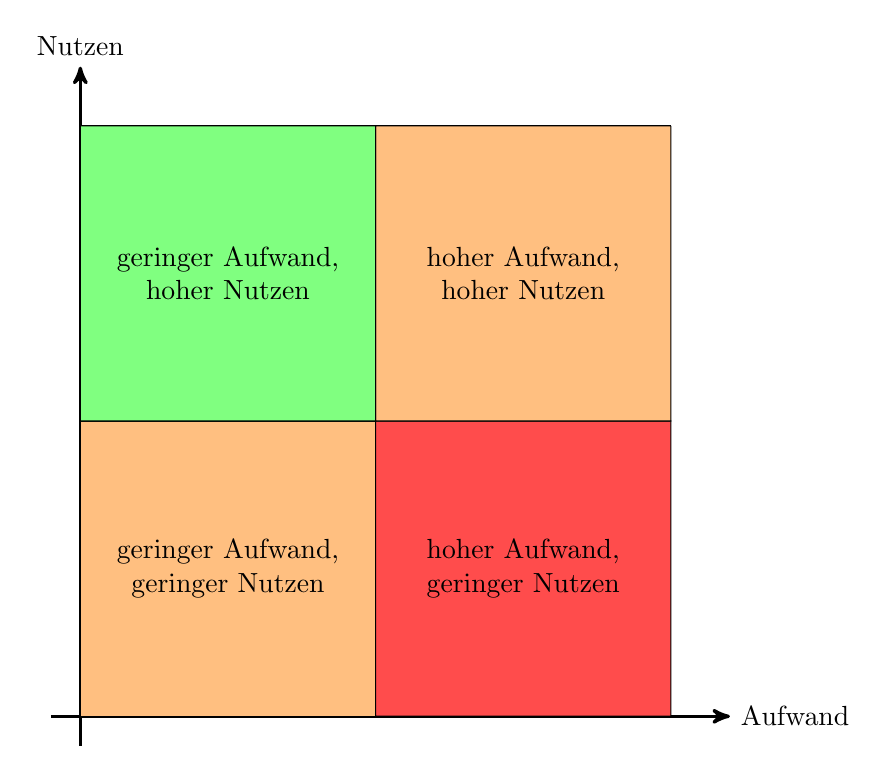
\begin{tikzpicture}[
    scale=5,
    axis/.style={very thick, ->, >=stealth'},
    important line/.style={thick},
    dashed line/.style={dashed, thin},
    pile/.style={thick, ->, >=stealth', shorten <=2pt, shorten
    >=2pt},
    text/.style={},
    every node/.style={color=black}
    ]

\newcommand{\size}{1.5}
\coordinate (SW) at (0,0);
\coordinate (SE) at (\size,0);
\coordinate (NW) at (0,\size);
\coordinate (NE) at (\size,\size);

% axis
\draw[axis] (-0.05*\size,0)  -- (1.1*\size,0) node(xline)[right]
        {Aufwand};
\draw[axis] (0,-0.05*\size) -- (0,1.1*\size) node(yline)[above] {Nutzen};

\newcommand{\warning}{orange!50}
\newcommand{\alert}{red!70}
\newcommand{\good}{green!50}

\draw[fill=\warning] (SW) -- (0.5*\size,0) -- (0.5*\size,0.5*\size) -- 
(0,0.5*\size) -- (SW); 


\draw[fill=\alert] (SE) -- (\size,0.5*\size) -- 
(0.5*\size,0.5*\size) -- (0.5*\size,0) -- (SE);
\draw[fill=\warning] (NE) -- (0.5*\size,\size) -- (0.5*\size,0.5*\size) -- 
(\size,0.5*\size) -- (NE);
\draw[fill=\good] (NW) -- (0.5*\size,\size) -- (0.5*\size,0.5*\size) -- 
(0,0.5*\size) -- (NW);

\newcommand{\textWidthBox}{3.5cm}
\node[text width=\textWidthBox,text centered] (NEmsg) at 
(0.75*\size,0.75*\size) 
	{hoher Aufwand,\\hoher Nutzen};
\node[text width=\textWidthBox,text centered] (NWmsg) at (0.25*\size,0.75*\size)
	{geringer Aufwand,\\hoher Nutzen};
\node[text width=\textWidthBox,text centered] (SEmsg) at (0.75*\size,0.25*\size)
	{hoher Aufwand,\\geringer Nutzen};
\node[text width=\textWidthBox,text centered] (SWmsg) at 
(0.25*\size,0.25*\size)
	{geringer Aufwand,\\geringer Nutzen};


\end{tikzpicture}
}
\caption{Kosten-Nutzen-Analyse der Anforderungen}
\label{fig:kosten-nutzen}
\end{center}
\end{figure}
